\documentclass{article}\usepackage[]{graphicx}\usepackage[]{xcolor}
% maxwidth is the original width if it is less than linewidth
% otherwise use linewidth (to make sure the graphics do not exceed the margin)
\makeatletter
\def\maxwidth{ %
  \ifdim\Gin@nat@width>\linewidth
    \linewidth
  \else
    \Gin@nat@width
  \fi
}
\makeatother

\definecolor{fgcolor}{rgb}{0.345, 0.345, 0.345}
\newcommand{\hlnum}[1]{\textcolor[rgb]{0.686,0.059,0.569}{#1}}%
\newcommand{\hlsng}[1]{\textcolor[rgb]{0.192,0.494,0.8}{#1}}%
\newcommand{\hlcom}[1]{\textcolor[rgb]{0.678,0.584,0.686}{\textit{#1}}}%
\newcommand{\hlopt}[1]{\textcolor[rgb]{0,0,0}{#1}}%
\newcommand{\hldef}[1]{\textcolor[rgb]{0.345,0.345,0.345}{#1}}%
\newcommand{\hlkwa}[1]{\textcolor[rgb]{0.161,0.373,0.58}{\textbf{#1}}}%
\newcommand{\hlkwb}[1]{\textcolor[rgb]{0.69,0.353,0.396}{#1}}%
\newcommand{\hlkwc}[1]{\textcolor[rgb]{0.333,0.667,0.333}{#1}}%
\newcommand{\hlkwd}[1]{\textcolor[rgb]{0.737,0.353,0.396}{\textbf{#1}}}%
\let\hlipl\hlkwb

\usepackage{framed}
\makeatletter
\newenvironment{kframe}{%
 \def\at@end@of@kframe{}%
 \ifinner\ifhmode%
  \def\at@end@of@kframe{\end{minipage}}%
  \begin{minipage}{\columnwidth}%
 \fi\fi%
 \def\FrameCommand##1{\hskip\@totalleftmargin \hskip-\fboxsep
 \colorbox{shadecolor}{##1}\hskip-\fboxsep
     % There is no \\@totalrightmargin, so:
     \hskip-\linewidth \hskip-\@totalleftmargin \hskip\columnwidth}%
 \MakeFramed {\advance\hsize-\width
   \@totalleftmargin\z@ \linewidth\hsize
   \@setminipage}}%
 {\par\unskip\endMakeFramed%
 \at@end@of@kframe}
\makeatother

\definecolor{shadecolor}{rgb}{.97, .97, .97}
\definecolor{messagecolor}{rgb}{0, 0, 0}
\definecolor{warningcolor}{rgb}{1, 0, 1}
\definecolor{errorcolor}{rgb}{1, 0, 0}
\newenvironment{knitrout}{}{} % an empty environment to be redefined in TeX

\usepackage{alltt}
\usepackage{amsmath} %This allows me to use the align functionality.
                     %If you find yourself trying to replicate
                     %something you found online, ensure you're
                     %loading the necessary packages!
\usepackage{amsfonts}%Math font
\usepackage{graphicx}%For including graphics
\usepackage{hyperref}%For Hyperlinks
\usepackage[shortlabels]{enumitem}% For enumerated lists with labels specified
                                  % We had to run tlmgr_install("enumitem") in R
\hypersetup{colorlinks = true,citecolor=black} %set citations to have black (not green) color
\usepackage{natbib}        %For the bibliography
\setlength{\bibsep}{0pt plus 0.3ex}
\bibliographystyle{apalike}%For the bibliography
\usepackage[margin=0.50in]{geometry}
\usepackage{float}
\usepackage{multicol}

%fix for figures
\usepackage{caption}
\newenvironment{Figure}
  {\par\medskip\noindent\minipage{\linewidth}}
  {\endminipage\par\medskip}
\IfFileExists{upquote.sty}{\usepackage{upquote}}{}
\begin{document}

\vspace{-1in}
\title{Labs 7-9 -- MATH 240 -- Computational Statistics}

\author{
  Harrison Wolfe \\
  Colgate University  \\
  Math Department  \\
  {\tt hwolfe@colgate.edu}
}

\date{4/3/2025}

\maketitle

\begin{multicols}{2}
\begin{abstract}
In this lab we analyzed the beta distribution and it's real world application. We attempted to annalyze the unique attributes of the beta distribution and then display the results in graphs and tables to show how accurately we can use the beta distribution given a sample or how well we can estimate the population level properties like mean, variance and skewness using estimators. 
\end{abstract}

\noindent \textbf{Keywords:} Beta distribution; Estimation; Parameters; Probability Distributions

\section{Introduction}
The aim of this lab was to analyze several aspects of the beta distribution. We analyzed the parameters, alpha and beta, the properties of the distribution based on a population and sample. We also completed an example of a real world application of the beta distribution discussing death rates in various countries. 

\section{Density Functions and Parameters}
The probability density function or PDF of the beta distribution is based on the parameters alpha and beta. The exact formula for the beta distribution is given below:
\[
f(x; \alpha, \beta) = \frac{x^{\alpha-1}(1-x)^{\beta-1}}{\int_0^1 t^{\alpha-1}(1-t)^{\beta-1} \, dt} \cdot 1_{(0 < x < 1)},
\]
Some examples with density functions of different parameters can be seen below:
\begin{figure}[H]
\centering
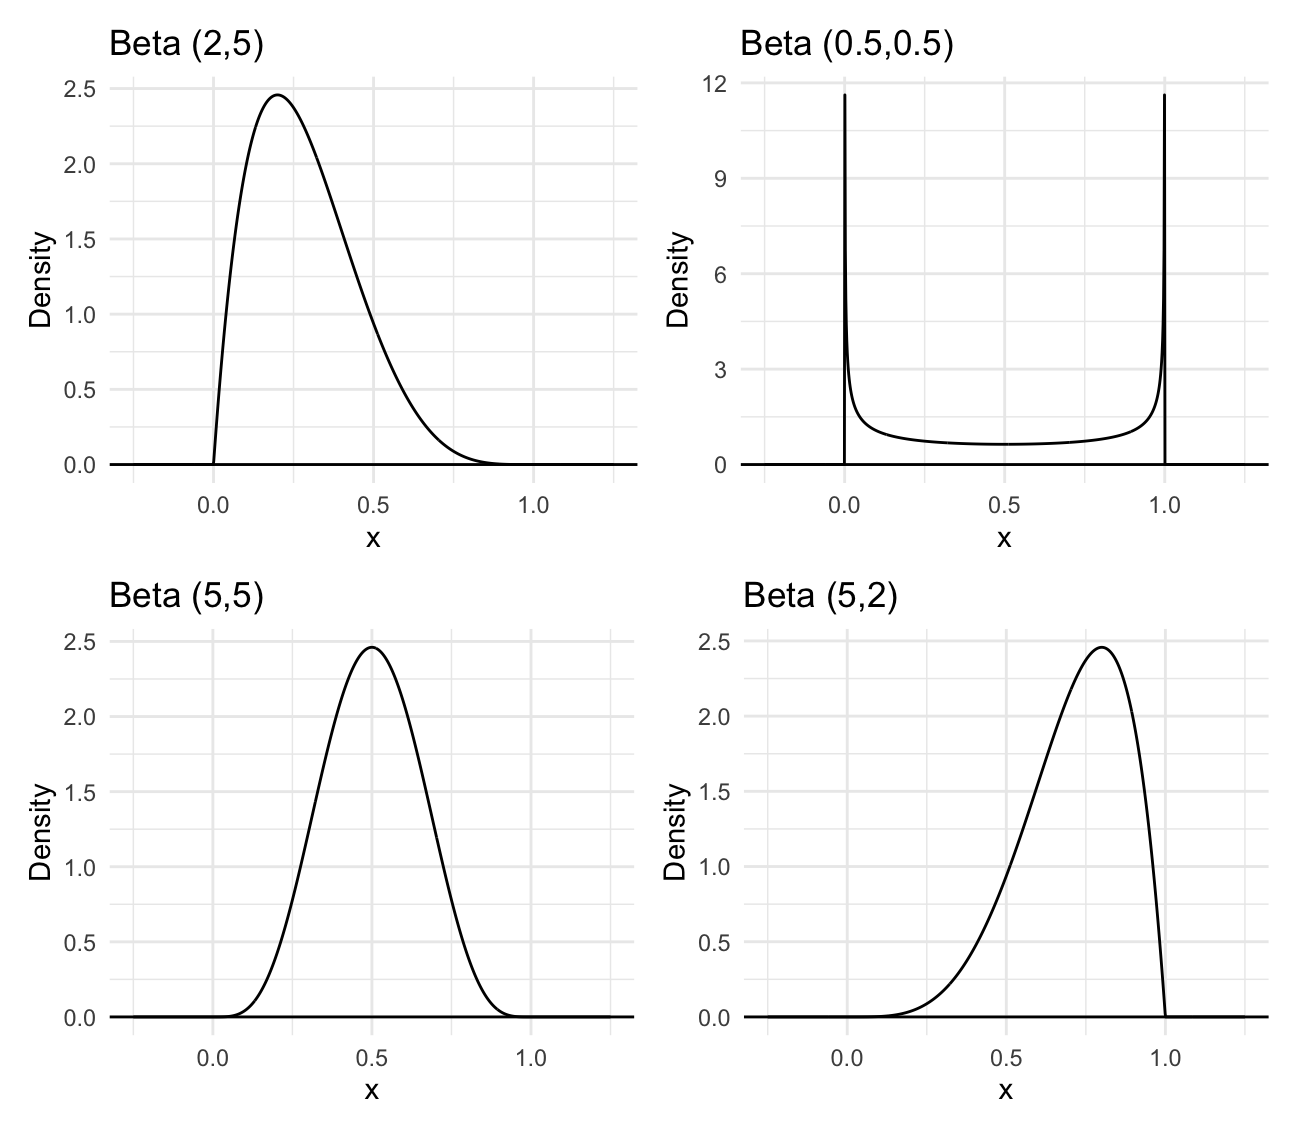
\includegraphics[width=0.47\textwidth]{BDistributions.png}  % Adjust the path and file name
\caption{Beta Distributions Given Different Parameters}
\label{Figure 1}
\end{figure}


\begin{figure}[H]
\centering
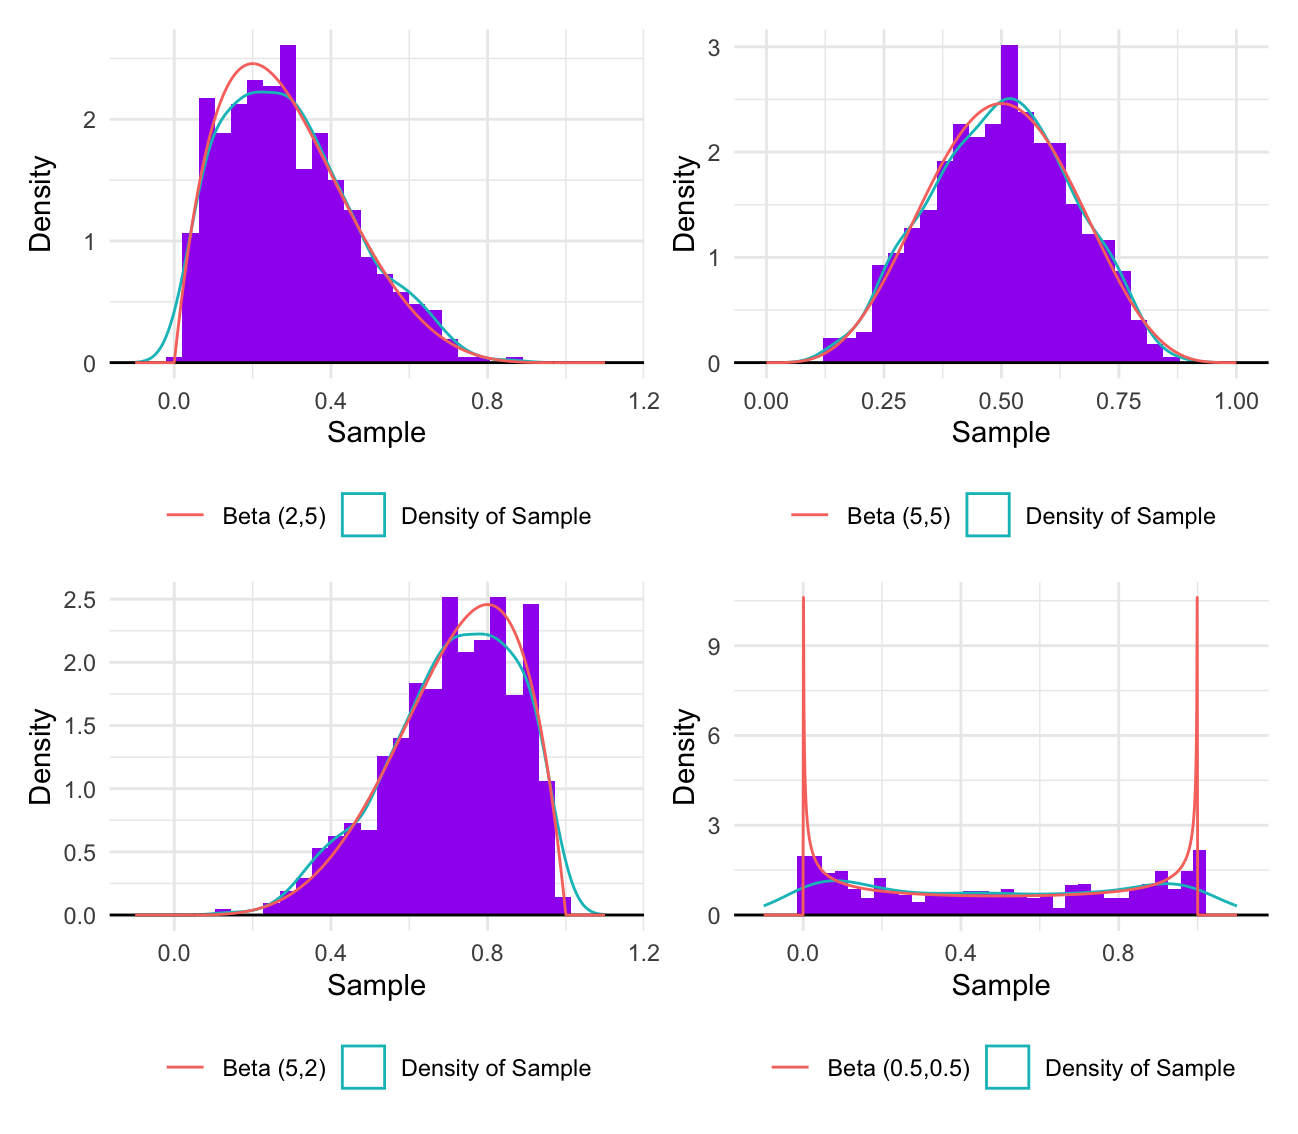
\includegraphics[width=0.47\textwidth]{SampDist}  % Adjust the path and file name
\caption{Samples of Beta Distributions}
\label{Figure 2}
\end{figure}


\begin{figure}[H]
\centering
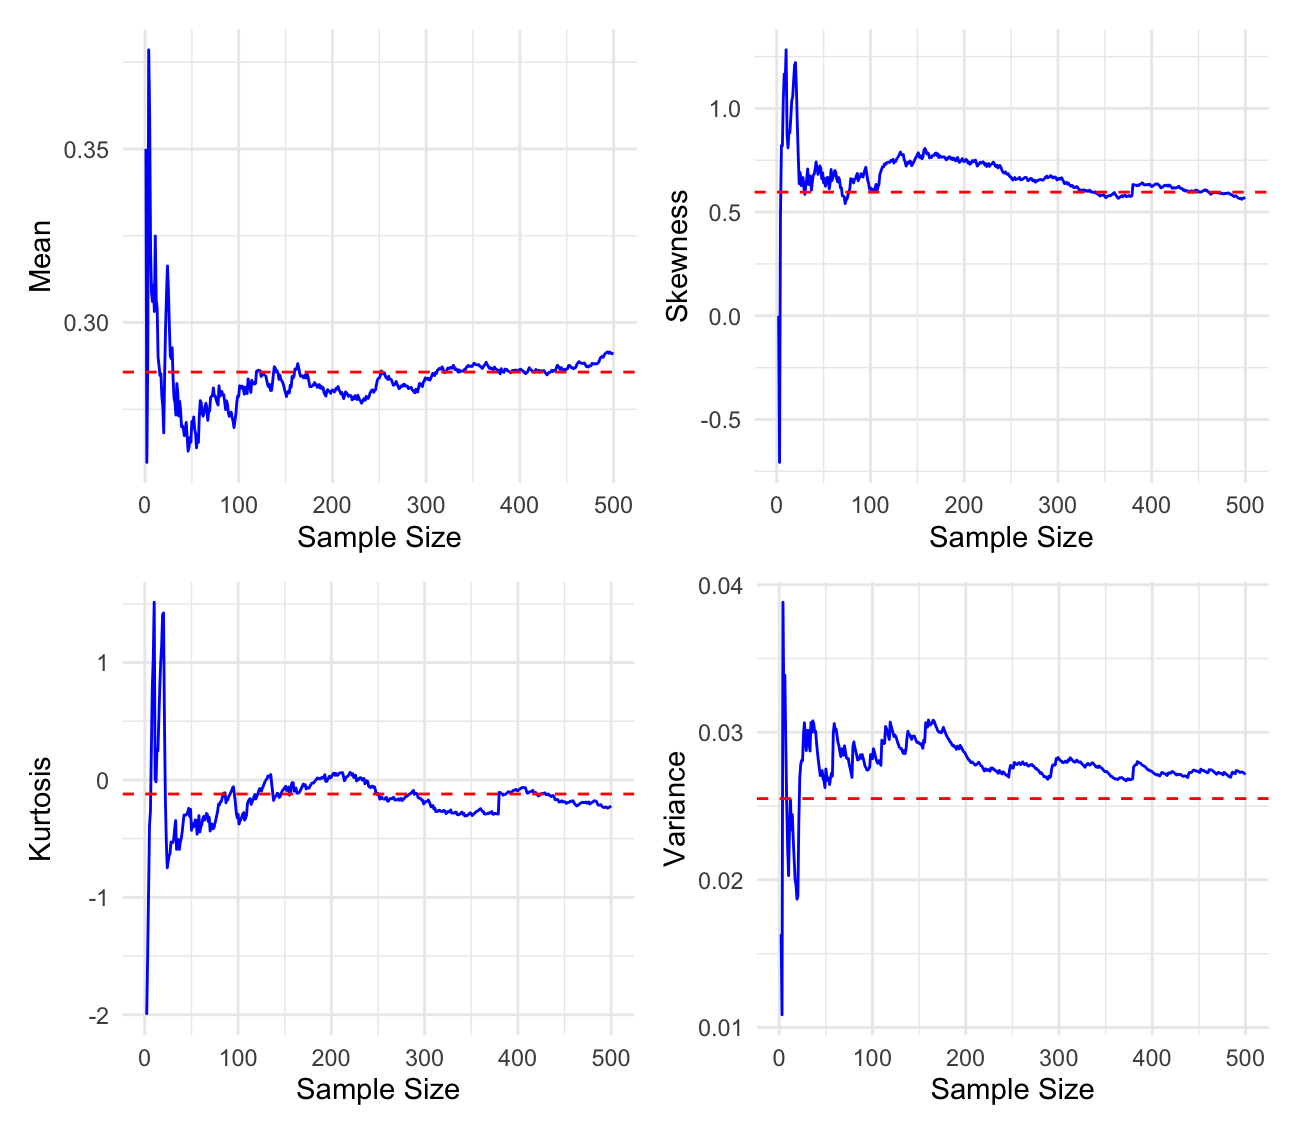
\includegraphics[width=0.47\textwidth]{SampStat}  % Adjust the path and file name
\caption{How Sample Size Effects Summary Stats}
\label{Figure 3}
\end{figure}

\begin{figure}[H]
\centering
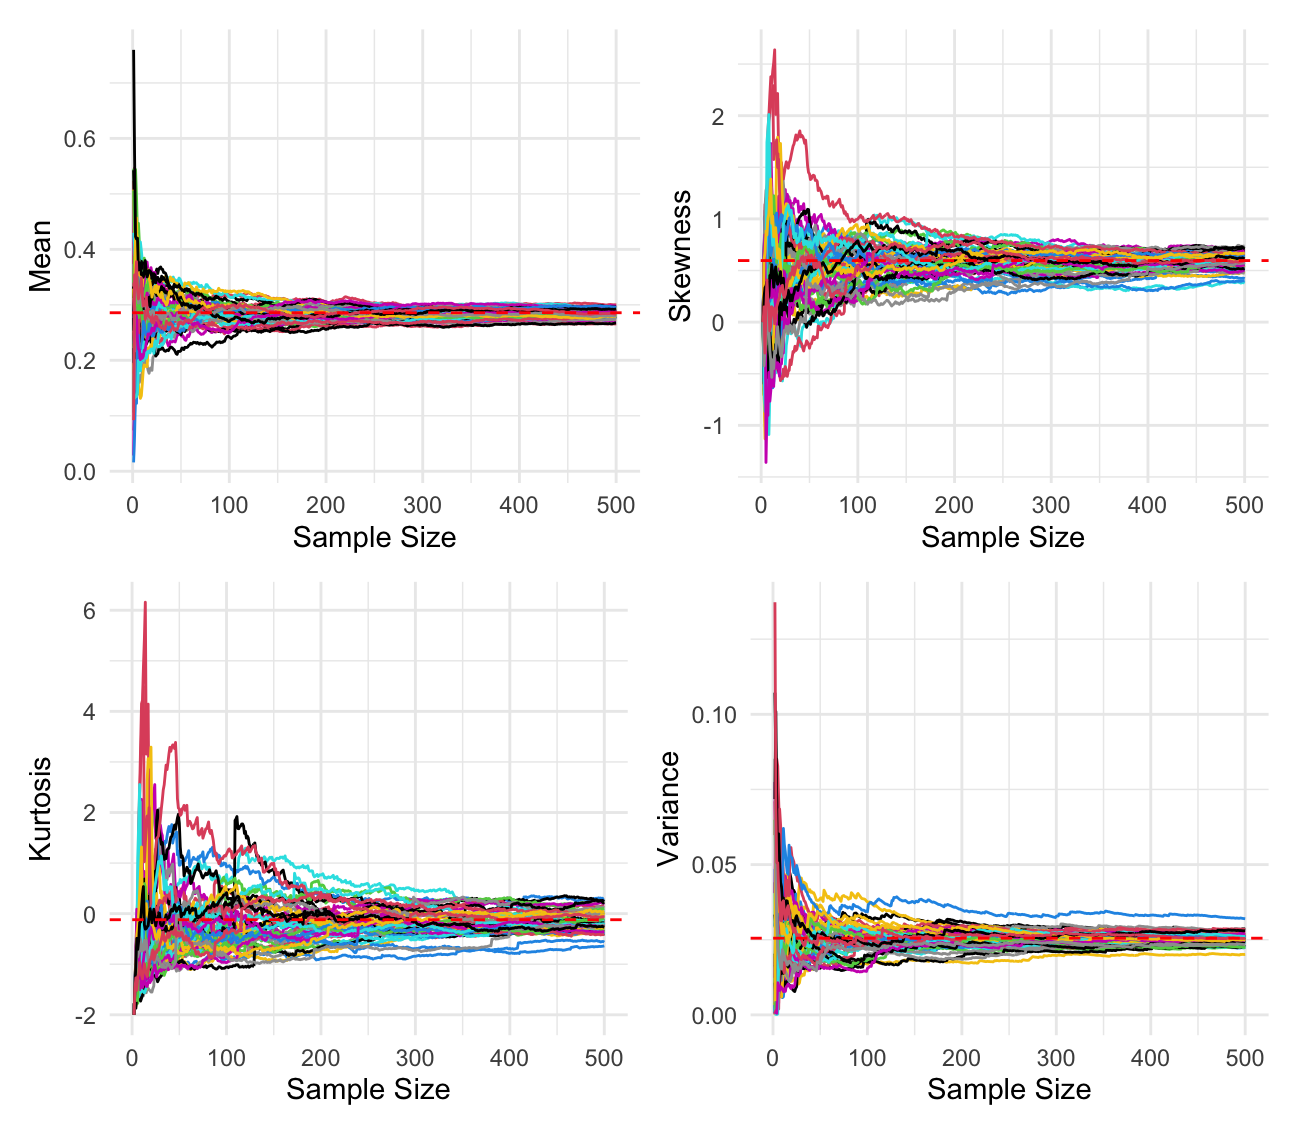
\includegraphics[width=0.47\textwidth]{SimpSampStat}  % Adjust the path and file name
\caption{How Sample Size Effects Summary Stats (Simulated)}
\label{Figure 4}
\end{figure}



\begin{figure}[H]
\centering
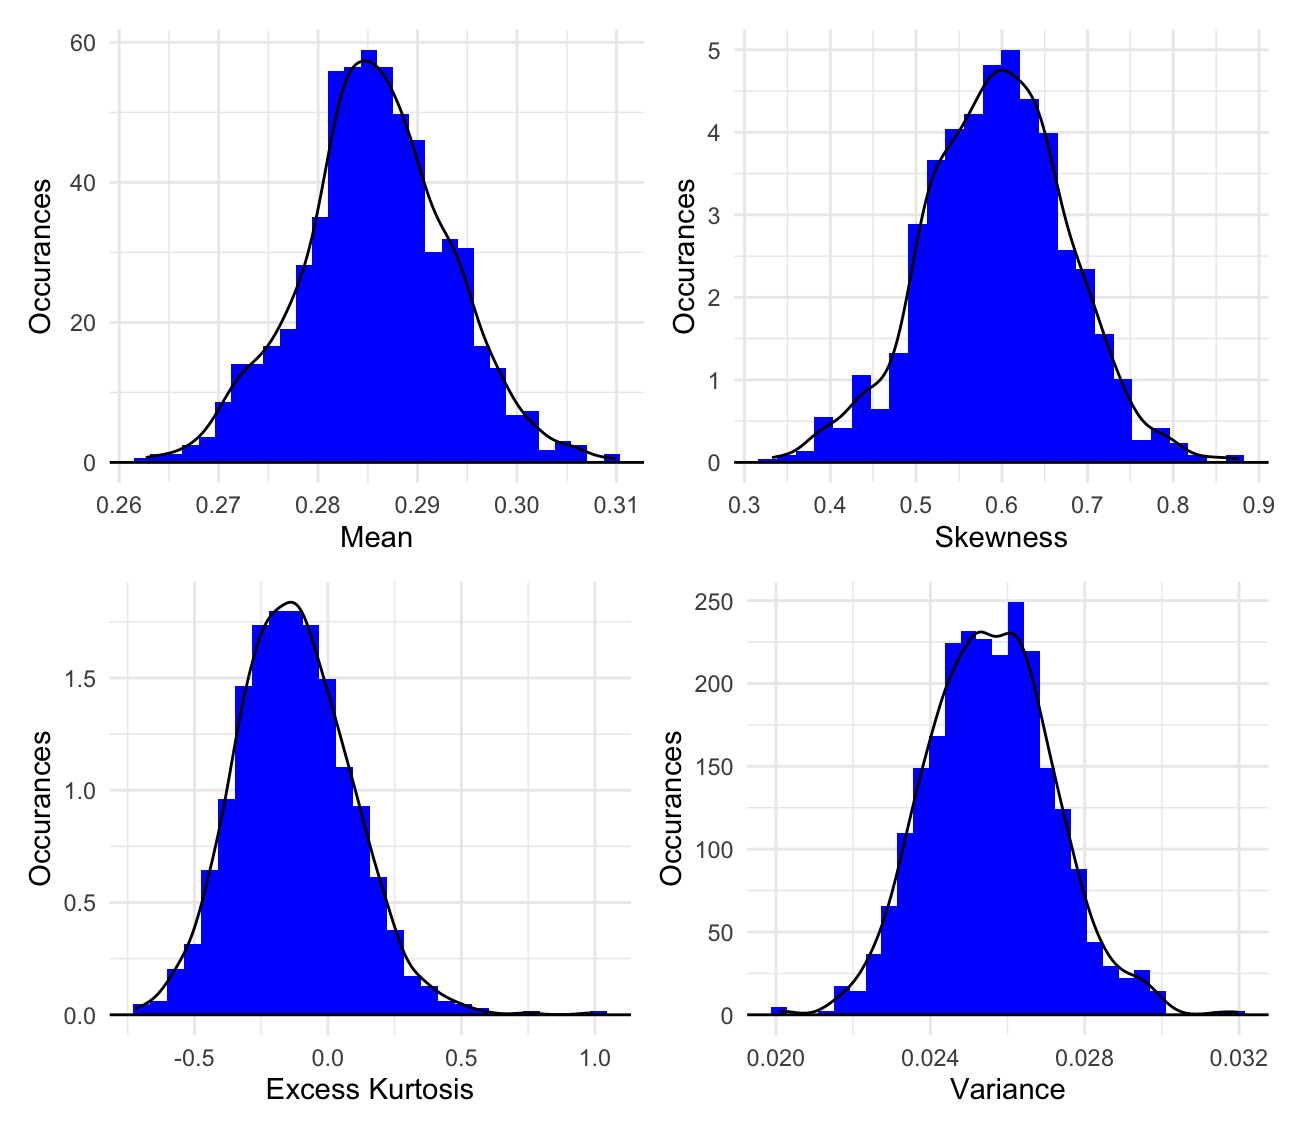
\includegraphics[width=0.47\textwidth]{StatDist}  % Adjust the path and file name
\caption{Sampling Distributions of Summary Statistics}
\label{Figure 5}
\end{figure}

\begin{figure}[H]
\centering
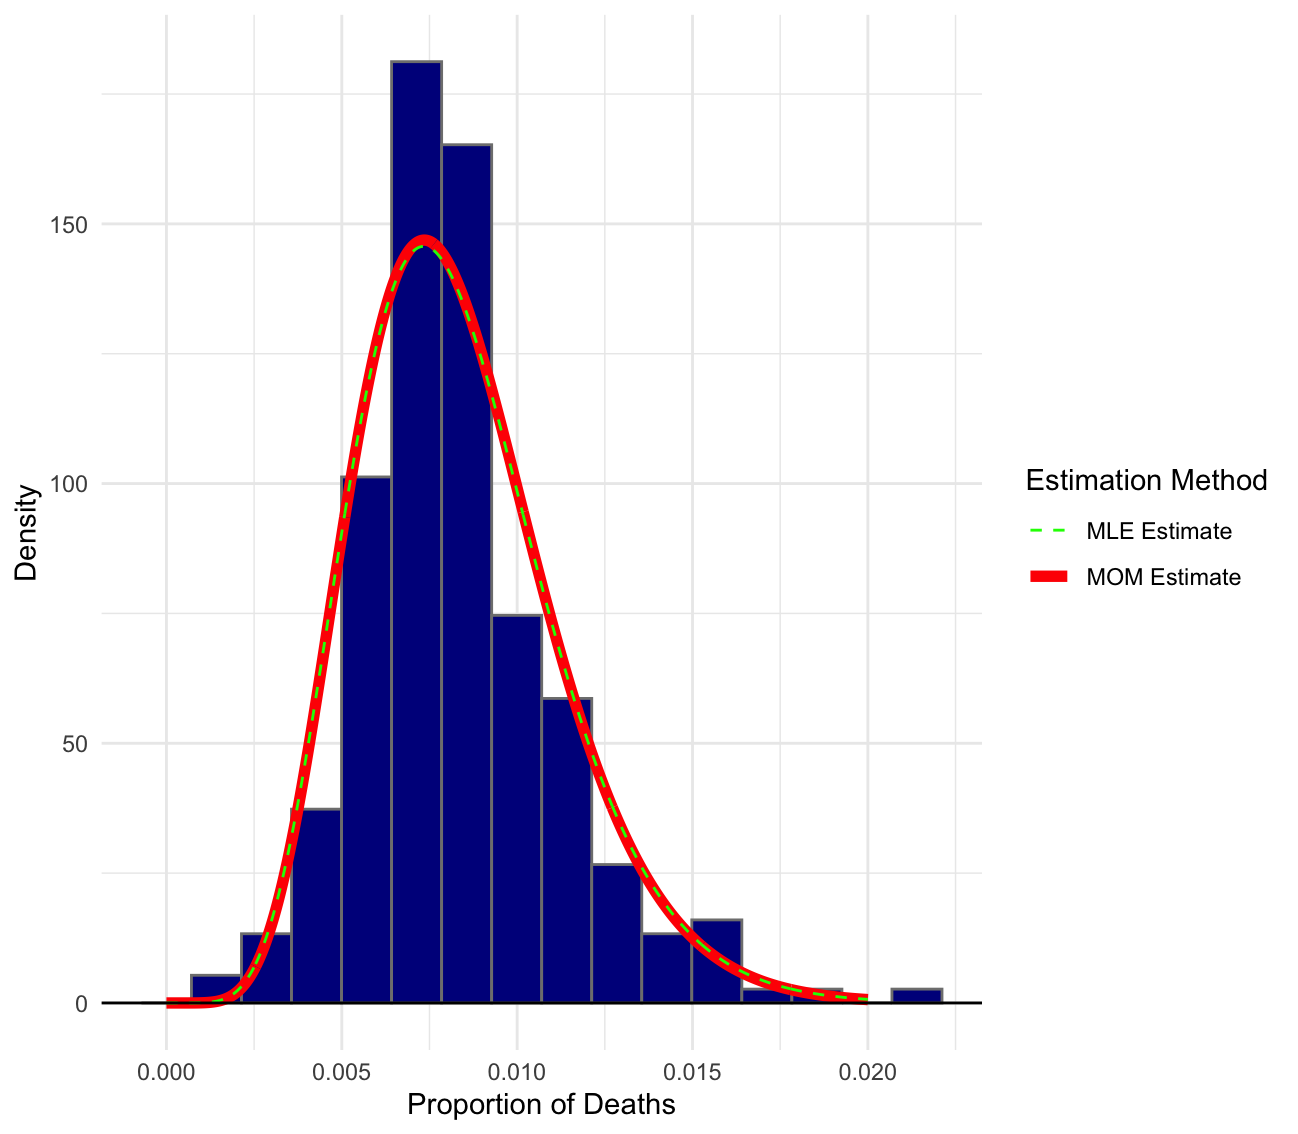
\includegraphics[width=0.47\textwidth]{EstiSamp}  % Adjust the path and file name
\caption{Superimposed Distributions with Estimates on Sample}
\label{Figure 6}
\end{figure}

\begin{figure}[H]
\centering
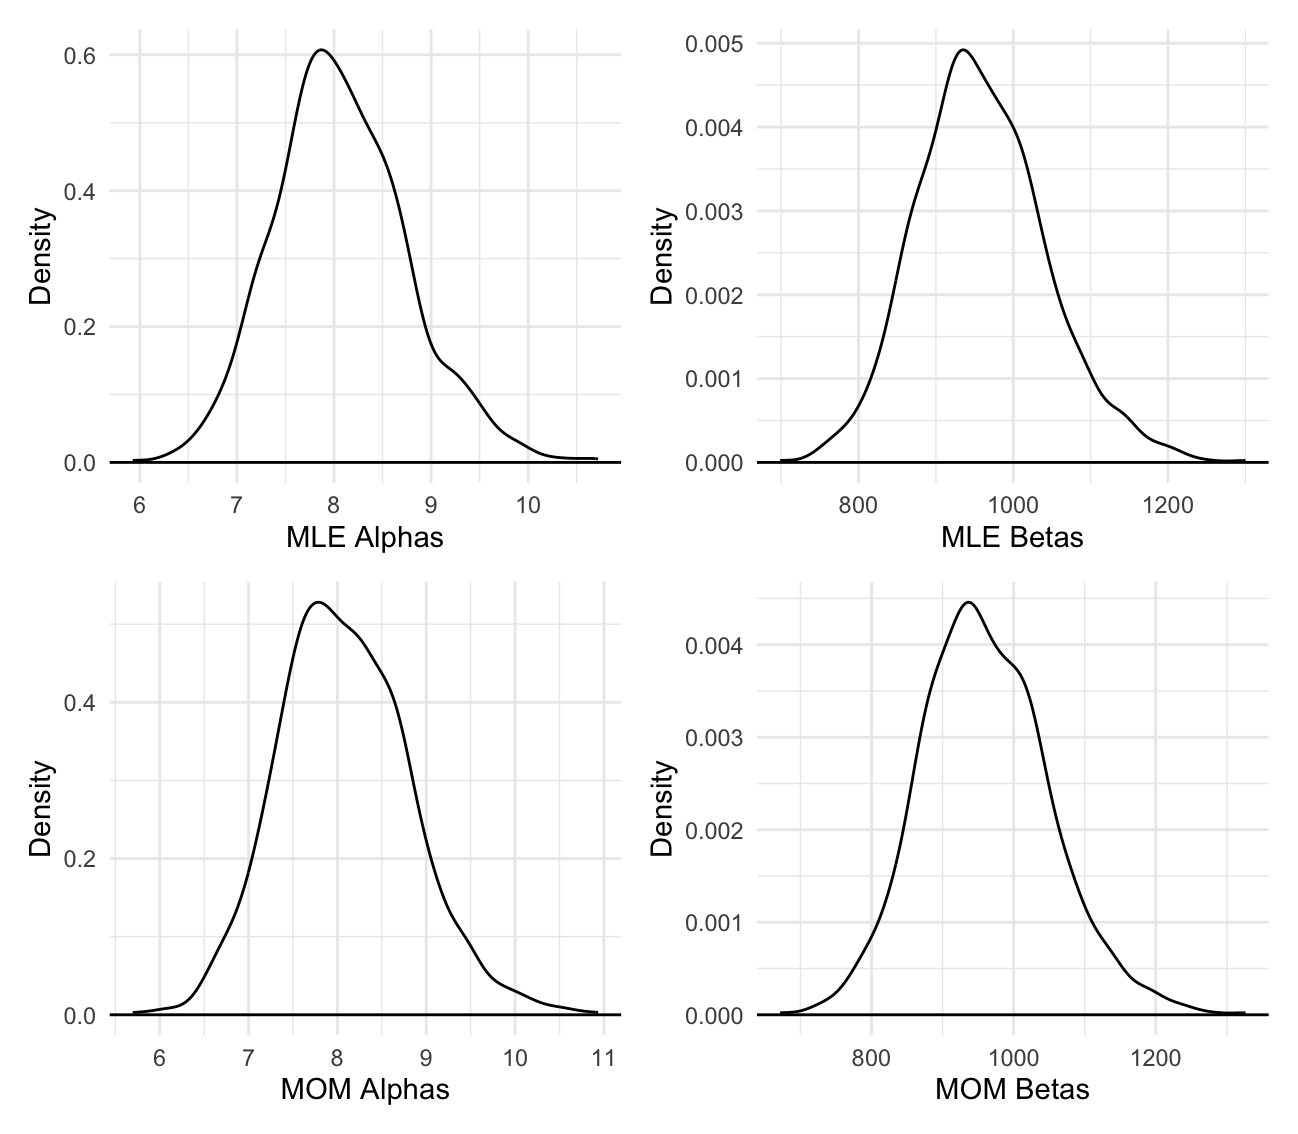
\includegraphics[width=0.47\textwidth]{SimuEsti}  % Adjust the path and file name
\caption{Simulated Estimators for Beta (8,950) Sample}
\label{Figure 7}
\end{figure}

\subsection{Intro Subsection}
You might need/want to discuss the topics in subsections. Or, you may have multiple questions.


\section{Methods}
Describe the data you are working with, if applicable. Describe the specific process you will follow to answer the question at hand. This does not mean you should write something like this.
\begin{quote}
\textit{I did this and then I did that and then I did this other thing and then..., and then..., and then...}
\end{quote}
Instead, it should provide a clear and concise narrative that flows from the problem specification in the Introduction to how you will approach answering it. This is where I would expect to see some citations for \texttt{R} packages you will use to conduct the statistical analysis reported in the Results section.


\subsection{Methods Subsection}
Much like the Introduction, subsections can be helpful for the Methods section. For example, you might describe data collection and the statistical analyses of the collected data in different subsections. Or, you may have different questions that require distinct methods. 

\section{Results}
Tie together the Introduction -- where you introduce the problem at hand -- and the methods --  what you propose to do to answer the question. Present your data, the results of your analyses, and how each reported aspect contributes to answering the question. This section should include table(s), statistic(s), and graphical displays. Make sure to put the results in a sensible order and that each result contributes a logical and developed solution. It should not just be a list. Avoid being repetitive. 

\subsection{Results Subsection}
Subsections can be helpful for the Results section, too. This can be particularly helpful if you have different questions to answer. 


\section{Discussion}
 You should objectively evaluate the evidence you found in the data. Do not embellish or wish-terpet (my made-up phase for making an interpretation you, or the researcher, wants to be true without the data \emph{actually} supporting it). Connect your findings to the existing information you provided in the Introduction.

Finally, provide some concluding remarks that tie together the entire paper. Think of the last part of the results as abstract-like. Tell the reader what they just consumed -- what's the takeaway message?

%%%%%%%%%%%%%%%%%%%%%%%%%%%%%%%%%%%%%%%%%%%%%%%%%%%%%%%%%%%%%%%%%%%%%%%%%%%%%%%%
% Bibliography
%%%%%%%%%%%%%%%%%%%%%%%%%%%%%%%%%%%%%%%%%%%%%%%%%%%%%%%%%%%%%%%%%%%%%%%%%%%%%%%%
\vspace{2em}

\noindent\textbf{Bibliography:} Note that when you add citations to your bib.bib file \emph{and}
you cite them in your document, the bibliography section will automatically populate here.

\begin{tiny}
\bibliography{bib}
\end{tiny}
\end{multicols}

%%%%%%%%%%%%%%%%%%%%%%%%%%%%%%%%%%%%%%%%%%%%%%%%%%%%%%%%%%%%%%%%%%%%%%%%%%%%%%%%
% Appendix
%%%%%%%%%%%%%%%%%%%%%%%%%%%%%%%%%%%%%%%%%%%%%%%%%%%%%%%%%%%%%%%%%%%%%%%%%%%%%%%%
\newpage
\onecolumn
\section{Appendix}


These figures could not fit in the margins of the template above so they have been placed here. Each graph was created using \texttt{ggplot2} and organized using \texttt{patchwork} \citep{ggplot} \citep{patchwork}. Each table was made using \texttt{xtable} \citep{xtable}. 



\begin{table}[ht]
\centering
\begin{tabular}{rrrrrrrl}
\hline
& Alpha & Beta & Mean & Variance & Skewness & Excess Kurtosis & Method \\ 
\hline
1 & 2.00 & 5.00 & 0.29 & 0.03 & 0.60 & -0.12 & Formula \\ 
2 & 5.00 & 5.00 & 0.50 & 0.02 & 0.00 & -0.46 & Formula \\ 
3 & 5.00 & 2.00 & 0.71 & 0.03 & -0.60 & -0.12 & Formula \\ 
4 & 0.50 & 0.50 & 0.50 & 0.12 & 0.00 & -1.50 & Formula \\ 
5 & 2.00 & 5.00 & 0.29 & 0.03 & 0.60 & -0.12 & Derived \\ 
6 & 5.00 & 5.00 & 0.50 & 0.02 & -0.00 & -0.46 & Derived \\ 
7 & 5.00 & 2.00 & 0.71 & 0.03 & -0.60 & -0.12 & Derived \\ 
8 & 0.50 & 0.50 & 0.50 & 0.12 & -0.00 & -1.50 & Derived \\ 
\hline
\end{tabular}
\caption{Summary Statistics Using Different Methods for the Beta Dist.}
\label{Table 1}
\end{table}


\begin{table}[ht]
\centering
\begin{tabular}{rlrrr}
  \hline
 & Names & Bias & Precision & MSE \\ 
  \hline
1 & Alpha MLE & 0.0720 & 2.1269 & 0.4754 \\ 
  2 & Alpha MOM & 0.0822 & 1.8286 & 0.5536 \\ 
  3 & Beta MLE & 9.1142 & 0.0001 & 7134.5577 \\ 
  4 & Beta MOM & 10.3424 & 0.0001 & 8290.0516 \\ 
   \hline
\end{tabular}
\caption{Predictors to determine how good our estimators are}
\label{Table 2}
\end{table}


\end{document}
